%************************************************
\chapter{Domain Name Service and Service Discovery}\label{ch:dns}
%************************************************
\textit{Topic 5: This chapter will present a brief introduction to Domain Name Service and Service Discovery. A short overview how to use these technology in cluster and cloud computing will be presented.} 
	
\section{DNS}
The Domain Name Service (DNS) is a service that allows humans readable language converting to IP address. In other word DNS allows to type names into the Web browser like www.youtube.com and automatically find that address on the Internet (IP), instead of type the IP-address of the web site.

The DNS organizes its servers into a hierarchy figure \ref{fig:DNShierarchy} shows the hierarchy. For the Internet, so-called root name servers reside at the top of the DNS hierarchy. The root servers are responsible for holding information about all the top level domains, it is the starting point for every name lookup operation. Top level domains are divided into two groups:

\begin{itemize}
	\item \textbf{Generic Top Level Domains (gTLD) .com, .edu, .net, .org, .mil etc.}
	\item \textbf{ Country Code Top Level Domain (ccTLD) e.g. .us, .ca, .tv , .uk etc.}
\end{itemize}
Each ccTLD identifies a particular country and is two letters long.   

\textbf{At the domain level or user DNS you have the resource you are looking for.??
}

\begin{figure}[bth]
	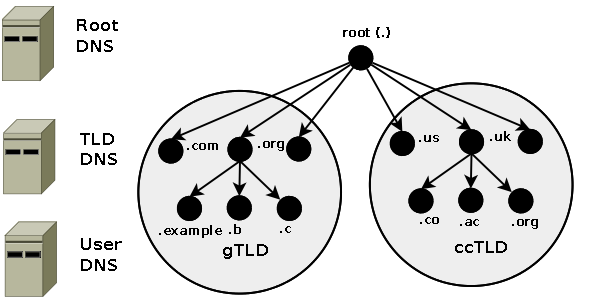
\includegraphics[width=1\linewidth]{gfx/DNShierarchy}
	\caption[routingtable]{DNS hierarchy} \label{fig:DNShierarchy}
\end{figure}

\textbf{Recursive Query Vs Iterative Query in DNS}

A recursive query is a kind of query, in which the DNS server, who received the query, will do the entire job fetching the answer, and giving it back to client. If DNS server is not able to resolve the requested query then it forwards the query to another DNS server until it gets an answer or the query fails.
In an iterative query, the name server, will not go and fetch the complete answer for the query. If the queried DNS server doesn't have an exact match for the queried name, the best possible information it can return is a referral, which might have the answer. The DNS client can then query the DNS server for which it obtained a referral.
\\\\
\textbf{Cached queries}

DNS caching allows any DNS server or client to locally store the DNS records and re-use them in the future. The Ip and domain is stored in local cache called stub-resolver for a period. By that, the overall network usage is reduced and thereby higher efficiency is achieved. The number of packets sent out also gets reduced and thereby a lower latency. 
\\\\
\textbf{How may Domain Name Services be beneficial in cluster and cloud computing?}


By having redundant Domain Name Services, the concept of single point of failure is avoided, in the case of failure of a single or multiple DNS services. Hence by having redundant DNS in cloud computing it becomes fault tolerant.  


To create additional resilience each root-server typically has multiple instances (copies) spread throughout the world. Each instance has the same IP address but data is sent to the closest instance using a process called anycasting.

\section{Service Discovery}
Service discovery protocols (SDP) are network protocols which allows automatic finding available services, on the same network. The service discovery requires a common language to allow software agents to make use of each other's services without the need for user intervention.


\textbf{Service Discovery in a Microservices Architecture}

The concern not having the service discovery in a microservices Architecture could for instance in the case of you have some code to invoke a service that has a REST API. To make a request on a specific service you need to know it's IP address and port number. In a cloud-based microservices application the problem occurs since the services runs inside the pods, and the pods have dynamically assigned IP addresses and Ports. The reason why pods have dynamically network location is based on failures, upgrades and auto-scaling. There are two service discovery patterns called client-side discovery and server-side discovery, to solve the issue described above.         

\textbf{The client-Side Discovery Pattern}

One of the approaches to service discovery is the client-side discovery pattern. In the client-side pattern the client has the responsibility of determining the network locations of available services, and furthermore has the responsibility of "load-balancing" requests. In the service registry the client can query for available services. The service registry then return a list of available services to the client, by using the load-balancing algorithm. Services periodontally send a heartbeat to the service registry to say "I'am alive". The network location for a specific service is removed from the service registry when it terminate. The client needs to have the business logic of the load-balancer, which is a cons that requires a lot of traffic on the client.

\textbf{The server-side discovery pattern}

The other approach to service discovery is the server-side discovery pattern. The approach is almost the same like in Client-Side Discovery Pattern, the difference is that client makes a request to service via load balancer, the load balancer then queries the service registry and return a list of available services to the load balancer. The load balancer then routes each request to the available service. The client only needs to concern to send requests to the load-balancer, and nothing else this is the pros of server-side discovery pattern.    Figure \ref{fig:ClienServerService} shows the differences between client-Side Discovery Pattern and the server-side discovery pattern  



\begin{figure}[bth]
	\centering
	\subfloat[client-Side Discovery Pattern]{{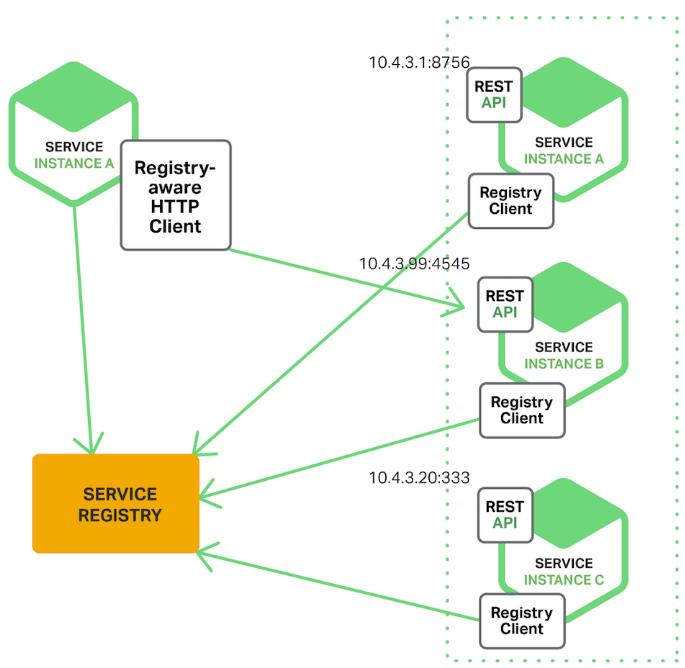
\includegraphics[width=4.1cm]{gfx/ClientSide} }}
	\qquad
	\subfloat[server-side discovery pattern]{{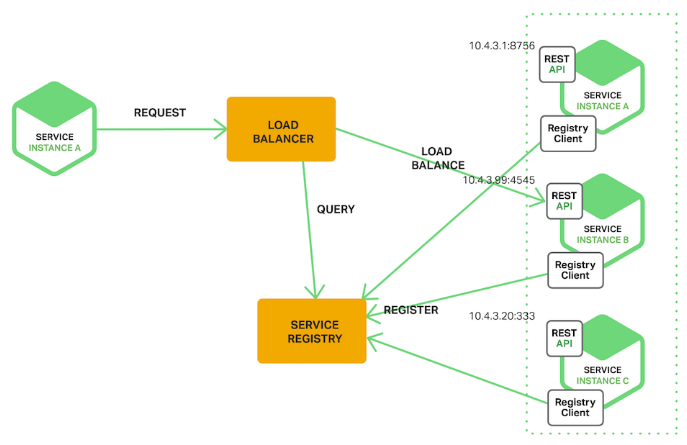
\includegraphics[width=6.2cm]{gfx/ServerSide} }}
	\caption{Client service discovery vs Server service discovery }
	\label{fig:ClienServerService}
\end{figure}



\textbf{How may Service Discovery be beneficial in cluster and cloud computing?}  
like described above, the server-side discovery pattern is used in Cloud computing. The way of register the services in service register and then send a list of available services on the cluster to load-balancer, while the load-balancer find the available service for the client has proved to be efficient.   
